\section{Series de potencias. Series de Fourier. Ecuaciones diferenciales}
\subsection{Introducción}
Sea $(f_n)_n$ una sucesión de funciones reales definidas todas en un mismo intervalo $I$ de la recta real. Para cada punto $x\in I$ tendremos una sucesión de números reales $(f_n(x))_n$ y también podemos considerar la serie numérica $\sum f_n(x)$ correspondiente. Supongamos que esta serie es convergente para todos los puntos $x$ de un cierto subconjunto de $M$ del intervalo $I$. Haciendo corresponder a cada $x\in M$ el valor $S(x)$ de la suma de la serie $\sum f_n(x)$, tendremos definida una nueva función en el conjunto $M$, que llamaremos función suma de la serie de funciones $\sum f_n$. El conjunto $M$ de todos los puntos en los cuales la serie es convergente se llama campo de convergencia de la serie funcional $\sum f_n$.
\begin{itemize}[label=\color{red}\textbullet, leftmargin=*]
	\item \color{lightblue}Ejemplo
\end{itemize}
Consideremos la sucesión de funciones $(f_n)_n$ dada por $f_n(x)=x^n$. Para cada $x\in\mathbb{R}$ la serie numérica $\sum x^n$ es una serie geométrica de razón $x$. Si $|x|<1$, la serie es convergente, luego el intervalo $(-1,1)$ está contenido en el campo de convergencia de la serie $\sum f_n$. Si $|x|>1$, la serie es divergente. Para $x=1$ y $x=-1$ las series son divergente y no sumable respectivamente. Luego el campo de convergencia es el intervalo abierto $(-1,1)$.
\subsection{Convergencia puntual}
\begin{itemize}[label=\color{red}\textbullet, leftmargin=*]
	\item \color{lightblue}Definición
\end{itemize}
Sea $I$ un subconjunto de $\mathbb{R}$. Supongamos que para cada número natural $n$ está dada una función $f_n:I\rightarrow\mathbb{R}$; la aplicación $n\rightarrow f_n$ recibe el nombre de sucesión de funciones. La función $f_n$ asociada al número natural $n$ recibe el nombre de término $n$-ésimo de la sucesión.

Informalmente, una sucesión de funciones es una lista sin fin \[ f ,~f_2,~\hdots,~f_n,~\hdots \] de funciones definidas en el punto $I$. Para cada punto $x\in I$ podemos considerar la sucesión de números reales que tiene por término $n$-ésimo real $f_n(x)$, valor en $x$ de la función $f_n$. Esta sucesión podrá ser convergente o no.
\begin{itemize}[label=\color{red}\textbullet, leftmargin=*]
	\item \color{lightblue}Definición
\end{itemize}
Sea $(f_n)_n$ una sucesión de funciones definidas en el conjunto $I,M$ un subconjunto de $I$ y $f$ una función definida en $M$. Si para cada $x\in M,f(x)=\lim_{n\to\infty}f_n(x)$, se dice que la sucesión $(f_n)_n$ convergente puntualmente a $f$ en $M$, o que converge punto a punto a $f$ en $M$. Cuando existe tal función $f$, decimos que la sucesión $(f_n)_n$ es convergente punto a punto en $M$, o que la sucesión $(f_n)$ es convergente puntualmente en $M$.
\begin{itemize}[label=\color{red}\textbullet, leftmargin=*]
	\item \color{lightblue}Ejemplo
\end{itemize}
La sucesión $(x^n)_n$ converge puntualmente en el intervalo cerrado $ [0,1]$ a la función $f$ definida en dicho intervalo por \[ f(x)=\left\{\begin{array}{ll}
	0 & \text{si }0\le x <1\\
	1 & \text{si }x=1
\end{array}\right. . \]

\begin{figure}
	\centering
	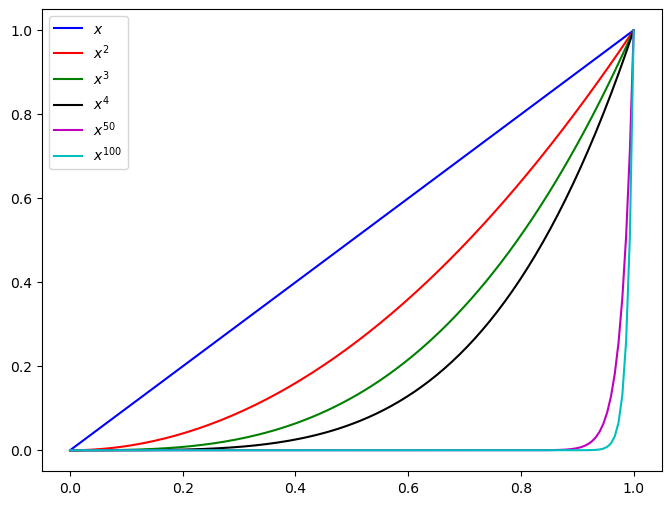
\includegraphics{"Temas/Tema 4/Gráfica 1.png"}
\end{figure}


\begin{itemize}[label=\color{red}\textbullet, leftmargin=*]
	\item \color{lightblue}Ejemplo
\end{itemize}
La sucesión $\left(\dfrac{x^n}{1+x^n}\right)_n$ converge puntualmente en el intervalo cerrado $[0,+\infty)$ a la función $f$ definida en tal intervalo por \[ f(x)=\left\{\begin{array}{ll}
	0 & \text{si }0\le x <1\\
	\frac{1}{2} & \text{si }x=1\\
	1 & \text{si } x >1\\
\end{array}\right.. \]

\begin{figure}[h]
	\centering
	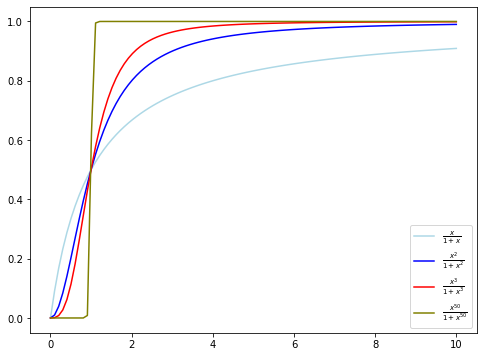
\includegraphics[width=0.7\textwidth]{"Temas/Tema 4/Gráfica 2.png"}
\end{figure}


La convergencia puntual puede expresarse en términos similares a los de la convergencia de sucesiones numéricas.
\begin{itemize}[label=\color{red}\textbullet, leftmargin=*]
	\item \color{lightblue}Definición (Otra forma para definir la convergencia puntual)
\end{itemize}
Sea $(f_n)$ una sucesión de funciones definidas en un conjunto $I,M$ un subconjunto de $I,f$ una función definida en $M$. La sucesión $(f_n)$ converge puntualmente a $f$ en $M$ si y sólo si para cada $x\in M$ y para cada $\epsilon>0$ existe un $N=N(\epsilon,x)$ tal que siempre que $n>N(\epsilon,x)$ se verifica $|f_n(x)-f(x)|<\epsilon$.

Análogo para la condición de Cauchy.
\begin{itemize}[label=\color{red}\textbullet, leftmargin=*]
	\item \color{lightblue}Definición
\end{itemize}
Una serie de funciones $\sum_{n=1}^{\infty}f_n$ es un par ordenado de sucesiones de funciones $\left((f_n),(s_n)\right)$ relacionadas por la condición de que para cada $n\in\mathbb{N}$ es \[ s_n=f_1+f_2+\cdots+f_n. \] Para cada $n\in\mathbb{N}$, el término $n$-ésimo de la primera sucesión, $f_n$, recibe el nombre de término $n$-ésimo de la serie; el término $n$-ésimo de la segunda sucesión, $s_n$, funciones converge puntualmente a una función $f$ en un conjunto $M$ si lo hace la sucesión de sus sumas parciales. En tal caso, la función $f$ es la suma de la serie en el conjunto $M$.
\begin{itemize}[label=\color{red}\textbullet, leftmargin=*]
	\item \color{lightblue}Ejemplo
\end{itemize}
La serie de funciones $\sum_{n=1}^{\infty}x^{n-1}$ converge puntualmente en $(-1,1)$ y su suma es la función $f(x)=\dfrac{1}{1-x}$, si $-1<x<1$.
\subsection{Convergencia uniforme}
El estudio de las sucesiones de funciones abre al menos dos interesantes opciones: de un lado, podemos construir nuevas funciones como límites de funciones conocidas; de otro, podemos pensar en sustituir, en ciertos problemas, una función dada por funciones que la aproximan y que pueden tener un comportamiento mejor controlado respecto a la situación que nos interese. En cualquiera de los dos casos, la primera tareas es examinar qué propiedades de las funciones que forman la sucesión se traspasan a la función límite.
\begin{itemize}[label=\color{red}\textbullet, leftmargin=*]
	\item \color{lightblue}Definición
\end{itemize}
Sea $(f_n)$ una sucesión de funciones definidas en un conjunto $I,M$ un subconjunto de $I, f$ una función definida en $M$. Se dice que la sucesión $(f_n)$ converge uniformemente a $f$ en $M$ si para cada $\epsilon>0$ existe un $N=N(\epsilon)$, para todo $x\in M$ se verifica $\left|f_n(x)-f(x)\right|<\epsilon$.

Es obvio que toda sucesión $(f_n)$ que converge uniformemente a una función $f$ en $M$, también converge puntualmente a $f$ en $M$.
\subsection{Series de potencias}
\begin{itemize}[label=\color{red}\textbullet, leftmargin=*]
	\item \color{lightblue}Definición
\end{itemize}
Sea $(a_n)_n$ y $x_0\in\mathbb{R}$, se llama serie de potencias de centro $x_0$ y coeficientes $a_n$ a la serie funcional $\sum_{n=1}^{\infty}a_n(x-x_0)^n$.

Obsérvese que el campo de convergencia no es vacío pues la serie converge en $x_0$.
\subsubsection{Convergencia uniforme de las series de potencias}
\begin{itemize}[label=\color{red}\textbullet, leftmargin=*]
	\item \color{lightblue}Teorema
\end{itemize}
Sea la serie de potencias $\sum_{n=1}^{\infty}a_n(x-x_0)^n$, si $\dfrac{1}{\lim_{n\to\infty}\sqrt[n]{|a_n|}}=r>0$, entonces se verifica: 
\begin{enumerate}[label=\arabic*)]
	\item Para cada $x\in(x_0-r,x_0+r)$, la serie $\sum_{n=1}^{\infty}a_n(x-x_0)^n$ es absolutamente convergente.
	\item Para cada $x\in\mathbb{R}\backslash\left[x_0-r,x_0+r\right]$, la serie $\sum a_n(x-x_0)^n$ no converge.
	\item Si $x$ es tal que $|x-x_0|=r$, no se puede asegurar nada.
\end{enumerate}
A $r=\dfrac{1}{\lim_{n\to\infty}\sqrt[n]{|a_n|}}$ se le llama \textcolor{lightblue}{radio de convergencia de la serie}. También se puede utilizar para su cálculo el límite. \[ r=\lim_{n\to\infty}\left|\dfrac{a_n}{a_{n+1}}\right|, \] que coincide con el valor anterior. A $(x_0-R,x_0+R)$ se le llama \textcolor{lightblue}{dominio de convergencia} de la serie. Evidentemente, las series $\sum_{n=0}^{\infty}a_nx^n$ y $\sum_{n=0}^{\infty}a_n(x-x_0)^n$ tienen el mismo radio de convergencia.
\begin{itemize}[label=\color{red}\textbullet, leftmargin=*]
	\item \color{lightblue}Teorema
\end{itemize}
Sea la serie de potencias $\sum_{n=0}^{\infty}a_n(x-x_0)^n$ y $r>0$ su radio de convergencia. Entonces $\forall[a,b]\subset(x_0-r,x_0+r)$, la serie $\sum_{n=0}^{\infty}a_n(x-x_0)^n$ es uniformemente convergente en $[a,b]$.
\begin{itemize}[label=\color{red}\textbullet, leftmargin=*]
	\item \color{lightblue}Teorema
\end{itemize}
Sea la serie de potencias $\sum_{n=0}^{\infty}a_n(x-x_0)^n$ y $r>0$ su radio de convergencia. Si además es convergente en $x=x_0+r$ (o en $x=x_0-r$), entonces la serie es uniformemente convergente en $[a,x_0+r]$ (respectivamente, en $[x_0-r,a]$) siendo $a\in(x_0-r,x_0+r)$.
\subsubsection{Continuidad de una serie de potencias}
Como consecuencia de los resultados anteriores tenemos los siguientes teoremas para el caso de las series de potencias.
\begin{itemize}[label=\color{red}\textbullet, leftmargin=*]
	\item \color{lightblue}Teorema
\end{itemize}
Sea $\sum_{n=0}^{\infty}a_n(x-x_0)^n$ y $r>0$ su radio de convergencia. Si $f(x)=\sum_{n=0}^{\infty}a_{n}(x-x_0)^n$ es su función límite, es decir su suma para cada $x\in(x_0-r,\,x_0+r)$, entonces $f$ es continua en dicho intervalo. Si además la serie es convergente en $x=x_0+r$ (o en $x=x_0+r$), entonces su función límite es continua por la izquierda en $x=x_0+r$ (respectivamente por la derecha en $x=x_0-r$).
\subsubsection{Derivación de una serie de potencias}
\begin{itemize}[label=\color{red}\textbullet, leftmargin=*]
	\item \color{lightblue}Teorema
\end{itemize}
Sea la serie de potencias $\sum_{n=0}^{\infty}a_{n}(x-x_0)^n$ y $r>0$ su radio de convergencia. Si $f$ es su función límite en su dominio de convergencia, entonces $f$ es derivable en $(x_0-r,\,x_0+r)$, la serie $\sum_{n=1}^{\infty}na_n(x-x_0)^{n-1}$ tiene el mismo radio de convergencia $r$ y se verifica que \[ f'(x)=\sum_{n=1}^{\infty}na_n(x-x_0)^{n-1}\:\forall x\in(x_0-r,\,x_0+r). \]
Como corolario obtenemos el siguiente resultado:
\begin{itemize}[label=\color{red}\textbullet, leftmargin=*]
	\item \color{lightblue}Corolario
\end{itemize}
Se la serie de potencias $\sum_{n=0}^{\infty}a_n(x-x_0)^{n}$ y $r>0$ su radio de convergencia. Si $f$ es una función límite en su intervalo de convergencia, entonces para cada $k\in\N$ la serie \[ \sum_{n=k}^{\infty}n(n-1)\cdots(n-k+1)a_n(x-x_0)^{n-k} \]tiene el mismo radio de convergencia $r,\:f$ admite derivadas de todos los órdenes en $(x_0-r,\,x_0+r)$ y se verifica que \[ f^{k)}(x)=\sum_{n=k}^{\infty}n(n-1)\cdots(n-k+1)a_n(x-x_0)^{n-k}. \]
\subsubsection{Integración de una serie de potencias}
\begin{itemize}[label=\color{red}\textbullet, leftmargin=*]
	\item \color{lightblue}Teorema
\end{itemize}
Sea $\sum_{n=0}^{\infty}a_n(x-x_0)^n$ y $r>0$ su radio de convergencia. Entonces para cada $[a,b]\subset(x_0-r,x_0+r)$ se verifica: \[ \int_{a}^{b}\left(\sum_{n=0}^{\infty}a_n(x-x_0)^{n}\right)\dx=\sum_{n=0}^{\infty}\int_{a}^{b}a_n(x-x_0)^{n}\dx. \]En particular, si $x_0=0$, para cada $x$ tal que $|x|<r$ se verifica: \[\int_0^{x}\left(\sum_{n=0}^{\infty}a_nt^n\right)\dt=\sum_{n=0}^{\infty}\int_{0}^{x}a_{n}t^{n}\:\mathrm{d}t=\sum_{n=0}^{\infty} \frac{a_{n}}{n+1}x^{n+1}.\]

\bu{Ejemplo}

$\sum_{n=0}^{\infty}(-1)^nx^n=\frac{1}{x+1}$ para cada $x \in(-1,1)$, entonces $\sum_{n=0}^{\infty}(-1)^{n} \frac{x^{n+1}}{n+1}=\sum_{n=1}^{\infty}(-1)^{n+1} \frac{x^n}{n}=\log(1+x)$ para cada $x \in(-1,1)$. Como esta última serie converge para $x=1$, dado que en este caso se trata de $\sum_{n=1}^{\infty}(-1)^{n+1} \frac{1}{n}$, obtenemos que $\log(2)=\sum_{n=1}^{\infty}\frac{(-1)^{n+1}}{n}$

\subsubsection{Series de potencias y desarrollo de Taylor}

\begin{itemize}[label=\color{red}\textbullet, leftmargin=*]
	\item \color{lightblue}Teorema
\end{itemize}
Sea $\sum_{n=0}^{\infty}a_{n}(x-x_{0})^{n}$ y $r>0$ su radio de convergencia. Si $f$ es su función límite, es decir, $f(x)=\sum_{n=0}^{\infty}a_{n}(x-x_{0})^{n}$ para cada $x \in(x_{0}-r,\,x_{0}+r)$, entonces
$$
a_{n}=\frac{f^{n)}(x_{0})}{n!}
$$
para cada $n \in\mathbb{N}$.

Según este teorema toda serie de potencias con $r>0$ y centrada en $x_{0}$, en su intervalo de convergencia, resulta ser la serie de Taylor de la función límite $f(x)$. Como aplicación se obtiene que $e^{x}=\sum_{n=0}^{\infty} \frac{x^{n}}{n!}$.

\subsubsection{Desarrollos en series de funciones}
\begin{itemize}
\item $\sin(x)=\sum_{n=0}^{\infty} \frac{(-1)^{n}x^{2n+1}}{(2n+1)!}$ para cada $x \in\mathbb{R}$
\item $\cos(x)=\sum_{n=0}^{\infty} \frac{(-1)^{n}x^{2n}}{(2n)!}$ para cada $x \in\mathbb{R}$
\item $\log(1+x)=\sum_{n=0}^{\infty}\dfrac{(-1)^{n+1}x^{n}}{n}$ para cada $x\in(-1,1]$.
\item $(1+x)^{\alpha}=\sum_{n=0}^{\infty}\binom{\alpha}{n}x^{n}$ para cada $x \in(-1,1)$
\item $e^{x}=\sum_{n=0}^{\infty} \frac{x^{n}}{n!}$ para cada $x \in\mathbb{R}$
\end{itemize}
\subsubsection{Series de Fourier}
Una función $f$ se dice que es periódica de periodo $T$ si $f(x+T)=f(x)$ para cada $x \in\mathbb{R}$. De forma que podemos considerar el intervallo $[a,a+T)$.

Sea $f:\mathbb{R}\longrightarrow\mathbb{R}$ una función periódica de periodo $T$ integrable en el intervalo $[0,T]$. Se definen los coeficientes coseno y seno de Fourier de $f$
$$
\begin{array}{c}
a_{n}=\frac{2}{T}\int_{0}^{T}\cos\left( \frac{2\pi nt}{T} \right)f(t)\:\mathrm{d}t,\quad n=0,1,2,\dots \\
b_{n}=\frac{2}{T}\int_{0}^{T}\sin\left( \frac{2\pi nt}{T} \right) f(t)\:\mathrm{d}t,\quad n=1,2,\dots
\end{array}
$$
respectivamente.

Se llama frecuencia $\omega=\frac{2\pi}{T}$

Se llama polinomio de Fourier de orden $N$ de $f$ a
$$
S_{N}(t)=\frac{a_{0}}{2}+\sum_{n=1}^{N}\left( a_{n}\cos\left( \frac{2\pi nt}{T}\right)+b_{n}\sin\left( \frac{2\pi nt}{T}  \right) \right).
$$
Cuando $\lim_{ N \to \infty }S_{N}(t)$ es convergente se llama serie de Fourier de $f$ y
$$
f(t)=\lim_{ N \to \infty }S_{N}(t).
$$
El siguiente resultado recoge lo anterior
\begin{itemize}[label=\color{red}\textbullet, leftmargin=*]
	\item \color{lightblue}Teorema
\end{itemize}
Sea $f$ una función definida en toda la recta real, periódica de periodo $T$ y continua por secciones en todo intervalo de periodicidad. Si en un cierto punto $x\in\mathbb{R}$ existen y son finitos los dos límites
$$
\lim_{ t \to 0^{+} } \frac{f(x-t)-f(x^{+})}{t}
$$
y
$$
\lim_{ t \to 0^{-} }\frac{f(x-t)-f(x.^{-})}{-t},
$$
la serie de Fourier asociada a $f$ tiene como suma en el punto $x$ el número $\frac{f(x^{+})-f(x^{-})}{2}$.
\subsection{Ecuaciones diferenciales}
\subsubsection{Definiciones básicas}
Comenzamos con la definición de \textit{ecuación diferencial}.
\begin{itemize}[label=\color{red}\textbullet, leftmargin=*]
	\item \color{lightblue}Definición
\end{itemize}
Llamaremos ecuación diferencial de orden $n$ a un expresión de la forma:
$$
F(x,y,y',y'',\dots,y^{n)})=0,
$$
siendo $F$ una función real definida en un abierto $A\subset \mathbb{R}^{n+2}$ e $y(x)$ una función real de variable real $n$ veces derivable.

Tras la definición concluimos que una ecuación diferencial no es sino una expresión en la que aparece una \textit{variable independiente}, $x$ y una \textit{variable dependiente} de $x$, $y(x)$ y las derivadas de ésta última con respecto de $x$. Obsérvese que el \textit{orden} de la ecuación es el orden de la mayor derivada que aparece en la ecuación.
\begin{itemize}[label=\color{red}\textbullet, leftmargin=*]
	\item \color{lightblue}Definición
\end{itemize}
Dada una ecuación diferencial
$$
F(x,y',y'',\dots,y^{n)})=0,
$$
diremos que la función $y:(a,b)\longrightarrow\mathbb{R}$ es una solución de la ecuación diferencial si:
\begin{enumerate}[label=\arabic*)]
\item Existe la derivada $n$-ésima de $y$ para todo punto $x\in(a,b)$.
\item El vector $(x,y(x),y'(x),\dots,y^{n)}(x))\in A$ para cada $x\in(a,b)$.
\item $F(x,y(x),y'(x),\dots,y^{n)}(x))=0$ para cada $x\in(a,b)$
\end{enumerate}
En general dada una ecuación diferecial es posible que existan infinitas soluciones. Llamaos solución general de una ecuación diferencial al conjunto de todas las funciones que verifican dicha ecuación. En general, son familias $n$-paramétricas de curvas siendo $n$ el orden de la ecuación.

\bu{Ejemplo}

La solución general de la ecuación $y'-y=0$ es el conjunto de funciones $y=Ce^{x}$, que es una familia de funciones dependiente de un sólo parámetro.

En ocasiones nos interesa que la solución que buscamos verifique además una condiciones adicionales a las que denominaremos \textit{condiciones de contorno, condiciones iniciales} o \textit{Problema de Cauchy}. Consiste en añadir a una ecuación diferencial de orden $n$, $n$ datos adicionales correspondientes a los valores iniciales de la función y sus $n-1$ primeras derivadas, es decir, el problema,
$$
\begin{cases}
F(x,y,y',\dots,y^{n)})=0 \\
y(x_{0})=y_{0},y_{0}'=y_{1},\dots,y^{n-1)}(x_{0})=y_{n-1}
\end{cases}
$$
donde $x_{0},y_{0},\dots,y_{n-1}$ son números reales arbitrarios.
\subsection{Existencia y unicidad de soluciones}
El siguiente teorema nos garantiza la existencia y unicidad de la solución en un problema de condiciones iniciales.
\begin{itemize}[label=\color{red}\textbullet, leftmargin=*]
	\item \color{lightblue}Teorema
\end{itemize}
Si $\epsilon,\delta$ dos números reales positivos, $x_{0},\,y_{0}$, dos números reales arbitrarios, y $f:(-\epsilon+x_{0},x_{0}+\epsilon)\times(-\delta+y_{0},y_{0}+\delta)\to \mathbb{R}$ una función continua con $\frac{\partial f}{\partial y}$ continua. Entonces existen un número real positivo $\lambda$ y una función $y:(-\lambda+x_{0},x_{0}+\lambda)\to \mathbb{R}$ que es la única del problema de condiciones iniciales 
$$
\begin{cases}
y' & =f(x,y) \\
y(x_{0}) & =y_{0}
\end{cases}
$$
La importancia de este teorema radica en que permite determinar de forma sencilla cuando algunos problemas de condiciones iniciales tienen solución única.

\bu{Ejemplo}

El problema de Cauchy
$$
\begin{cases}
y'=x^{2}+y^{2}\\
y(0)=0
\end{cases}
$$
verifica las condiciones del teorema.
\subsection{Métodos para resolver ecuaciones diferenciales}
\subsubsection{Ecuaciones del tipo $y'=f(x)$}
El caso más sencillo de ecuaciones diferenciales que tenemos es aquel en el que no aparece explícitamente la incógnita $y$, es decir, se corresponden con el tipo $y'=f(x)$. Para resolverlas basta con integrar en cada miembro de la ecuación, obtenemos así,
$$
\begin{array}{l}
\int \:\mathrm{d}y=\int f(x)\:\mathrm{d}x \\
y=\int f(x)+C
\end{array}
$$
siendo $C$ una constante.

Una ecuación de primer orden se dice que es de variables separadas si tiene la forma 
$$
y'=f(y)g(x)
$$
donde $f$ y $g$ son dos funciones reales definidas sobre intervalos abiertos.

Suponiendo que $f(y)\neq 0$ en el dominio de definición de $f$ podemos transformar nuestra ecuación en la forma
$$
\frac{y'}{f(y)}=g(x),
$$
que nos proporciona una expresión de la ecuación con cada variable a un lado de la igualdad. Entonces, si somos capaces de calcular las primitivas
$$
\int \frac{y'(x)}{f(y(x))}\:\mathrm{d}x=\int g(x)\:\mathrm{d}x,
$$
habremos resuelto la ecuación inicial.

\bu{Ejemplo}

$$
y'=yx
$$
o lo que es lo mismo,
$$
\frac{y'}{y}=x,
$$
integrado la expresión anterior obtenemos
$$
\begin{array}{c}
\int \frac{y'(x)}{y(x)}\:\mathrm{d}x=\int x\:\mathrm{d}x \\
\log(y(x))+C_{1}=\frac{x^{2}}{2}+C_{2}.
\end{array}
$$
Despejando, finalmente queda que
$$
y(x)=e^{ \frac{x^{2}}{2} }\cdot e^{ C_{2}-C_{1} },
$$
llamando $K=e^{ C_{2}-C_{1} }$ obtenemos que la solución viene dada por

Cuando la ecuación diferencial viene dada de la forma $\frac{\:\mathrm{d}y}{\:\mathrm{d}x}=f(y)$, es decir, no depende de la variable $x$, se dice que la ecuación diferencial es \textbf{autónoma}. La ecuación logística es un ejemplo de este tipo de ecuaciones diferenciales. Esta ecuación describe la variación del tamaño de una población en la que el crecimiento per cápita es dependiente de la densidad. Si se denomina $N(t)$ al tamaño de la población en el instante $t$, entonces la variación del crecimiento está dada por el sistema 
$$
\frac{\:\mathrm{d}N}{\:\mathrm{d}t}=rN\left( 1-\frac{N}{K} \right)\quad \text{con }N(0)=N_{0},
$$
siendo $r$ y $K$ constantes positivas.

Resolviendo obtenemos la solución
$$
N(t)=\frac{K}{1-\left( \frac{K}{n_{0}}-1 \right)e^{ -rt }}.
$$
Obsérvese que $\lim_{ t \to \infty }N(t)=K$. Además $N(t)=0$ es una solución así como la solución $N(t)=K$ (puntos fijos).